
\documentclass[12pt,a4paper,titlepage]{article}
\usepackage{amsmath}
\usepackage{latexsym}
\usepackage{amssymb}
\usepackage{amstext}
\usepackage{nccmath}
\usepackage{mathtools}
\usepackage{array}
\usepackage{fixmath}
\usepackage{mathrsfs}
\usepackage{pdfpages}

\setlength{\textwidth}{15cm} \setcounter{page}{159}

\begin{document}


\begin{titlepage}
    \begin{center}
        \vspace*{3.5cm}
        
        \textbf{\huge{Programming Assignment}}
        \vspace{1cm}

        \textbf{\huge{Report}}

        \vspace{6cm}

        \begin{verse}
            \ \ \ \ \ \ \ \ \ \ \ \ \ \ \ \ \ \ \ \ \ \ \ \ \ \textbf{\large{Student: Zhiwei Han}}\\
            \ \ \ \ \ \ \ \ \ \ \ \ \ \ \ \ \ \ \ \ \ \ \ \ \ \textbf{\large{Matrikel Nr. 03672554
            }}\\
        \end{verse}


        
        \vspace{1cm}
        
%        \includegraphics[width=0.4\textwidth]{university} 
        
        Lehrstuhl f\"ur Datenverarbeitung\\
        Technische Universt\"at M\"unchen\\
        \today
        
    \end{center}
\end{titlepage}



\setlength{\parindent}{0pt} \setlength{\parskip}{2ex plus 0.5ex
minus 0.2ex}


\section*{1. Solution with Dynamic Programming}
\subsection*{1.1 Find a mapping to linearize the state space into a vector}
The approach is just to vectorize the 2D maze array and kick out the wall grids.
\subsection*{1.2 Visualize the optimal policy with a 2d plot, where colored boxes indicate the direction of the optimal action}
In order to optimize the visualization, legal states (not a wall or out of range) are denoted as starting points with arrows instead of color boxes and they also have actions, which denoted as arrows. The walls are denoted with blue squares.\\
(The Plots please see attachment 1.)
\subsection*{1.3 Do the two methods generate the same policy?}
Yes, from the graphs showed in attachment we know, that the optimal policies, derived from value iteration and policy iteration, are the optimal and same with proper parameter settings if they are both converged.

\section*{2. A Study of Algorithm Properties}
\subsection*{2.1 Vary the discounting factor $\alpha$. Does this have a influence on the final policy?}
Yes, discount factor $\alpha$ decides how further the algorithm looks into future. If it is too small, the algorithms cares only about the step cost instead of future state value and only the states near the goal state can obtain the right policy. In other words, the agent will more likely get lost in the states, which far from the terminal state.
\subsection*{2.2 Run policy evaluation, policy iteration and value iteration until each have converged. Regard the solution of those runs as the ground truth value function and policy.}
(The Plots please see attachment 3.)
\subsection*{2.3 Now run the three algorithms again and plot the error to the ground truth with respect to the iterations.}
(The Plots please see attachment 2.)
\subsection*{2.4 Run this error plot again for three sensible values of $\alpha$.}
(The Plots please see attachment 2.)
\newpage
\section*{Attachment}
\subsection*{1. Optimal policy plots according to different parameter setting}
\begin{center}
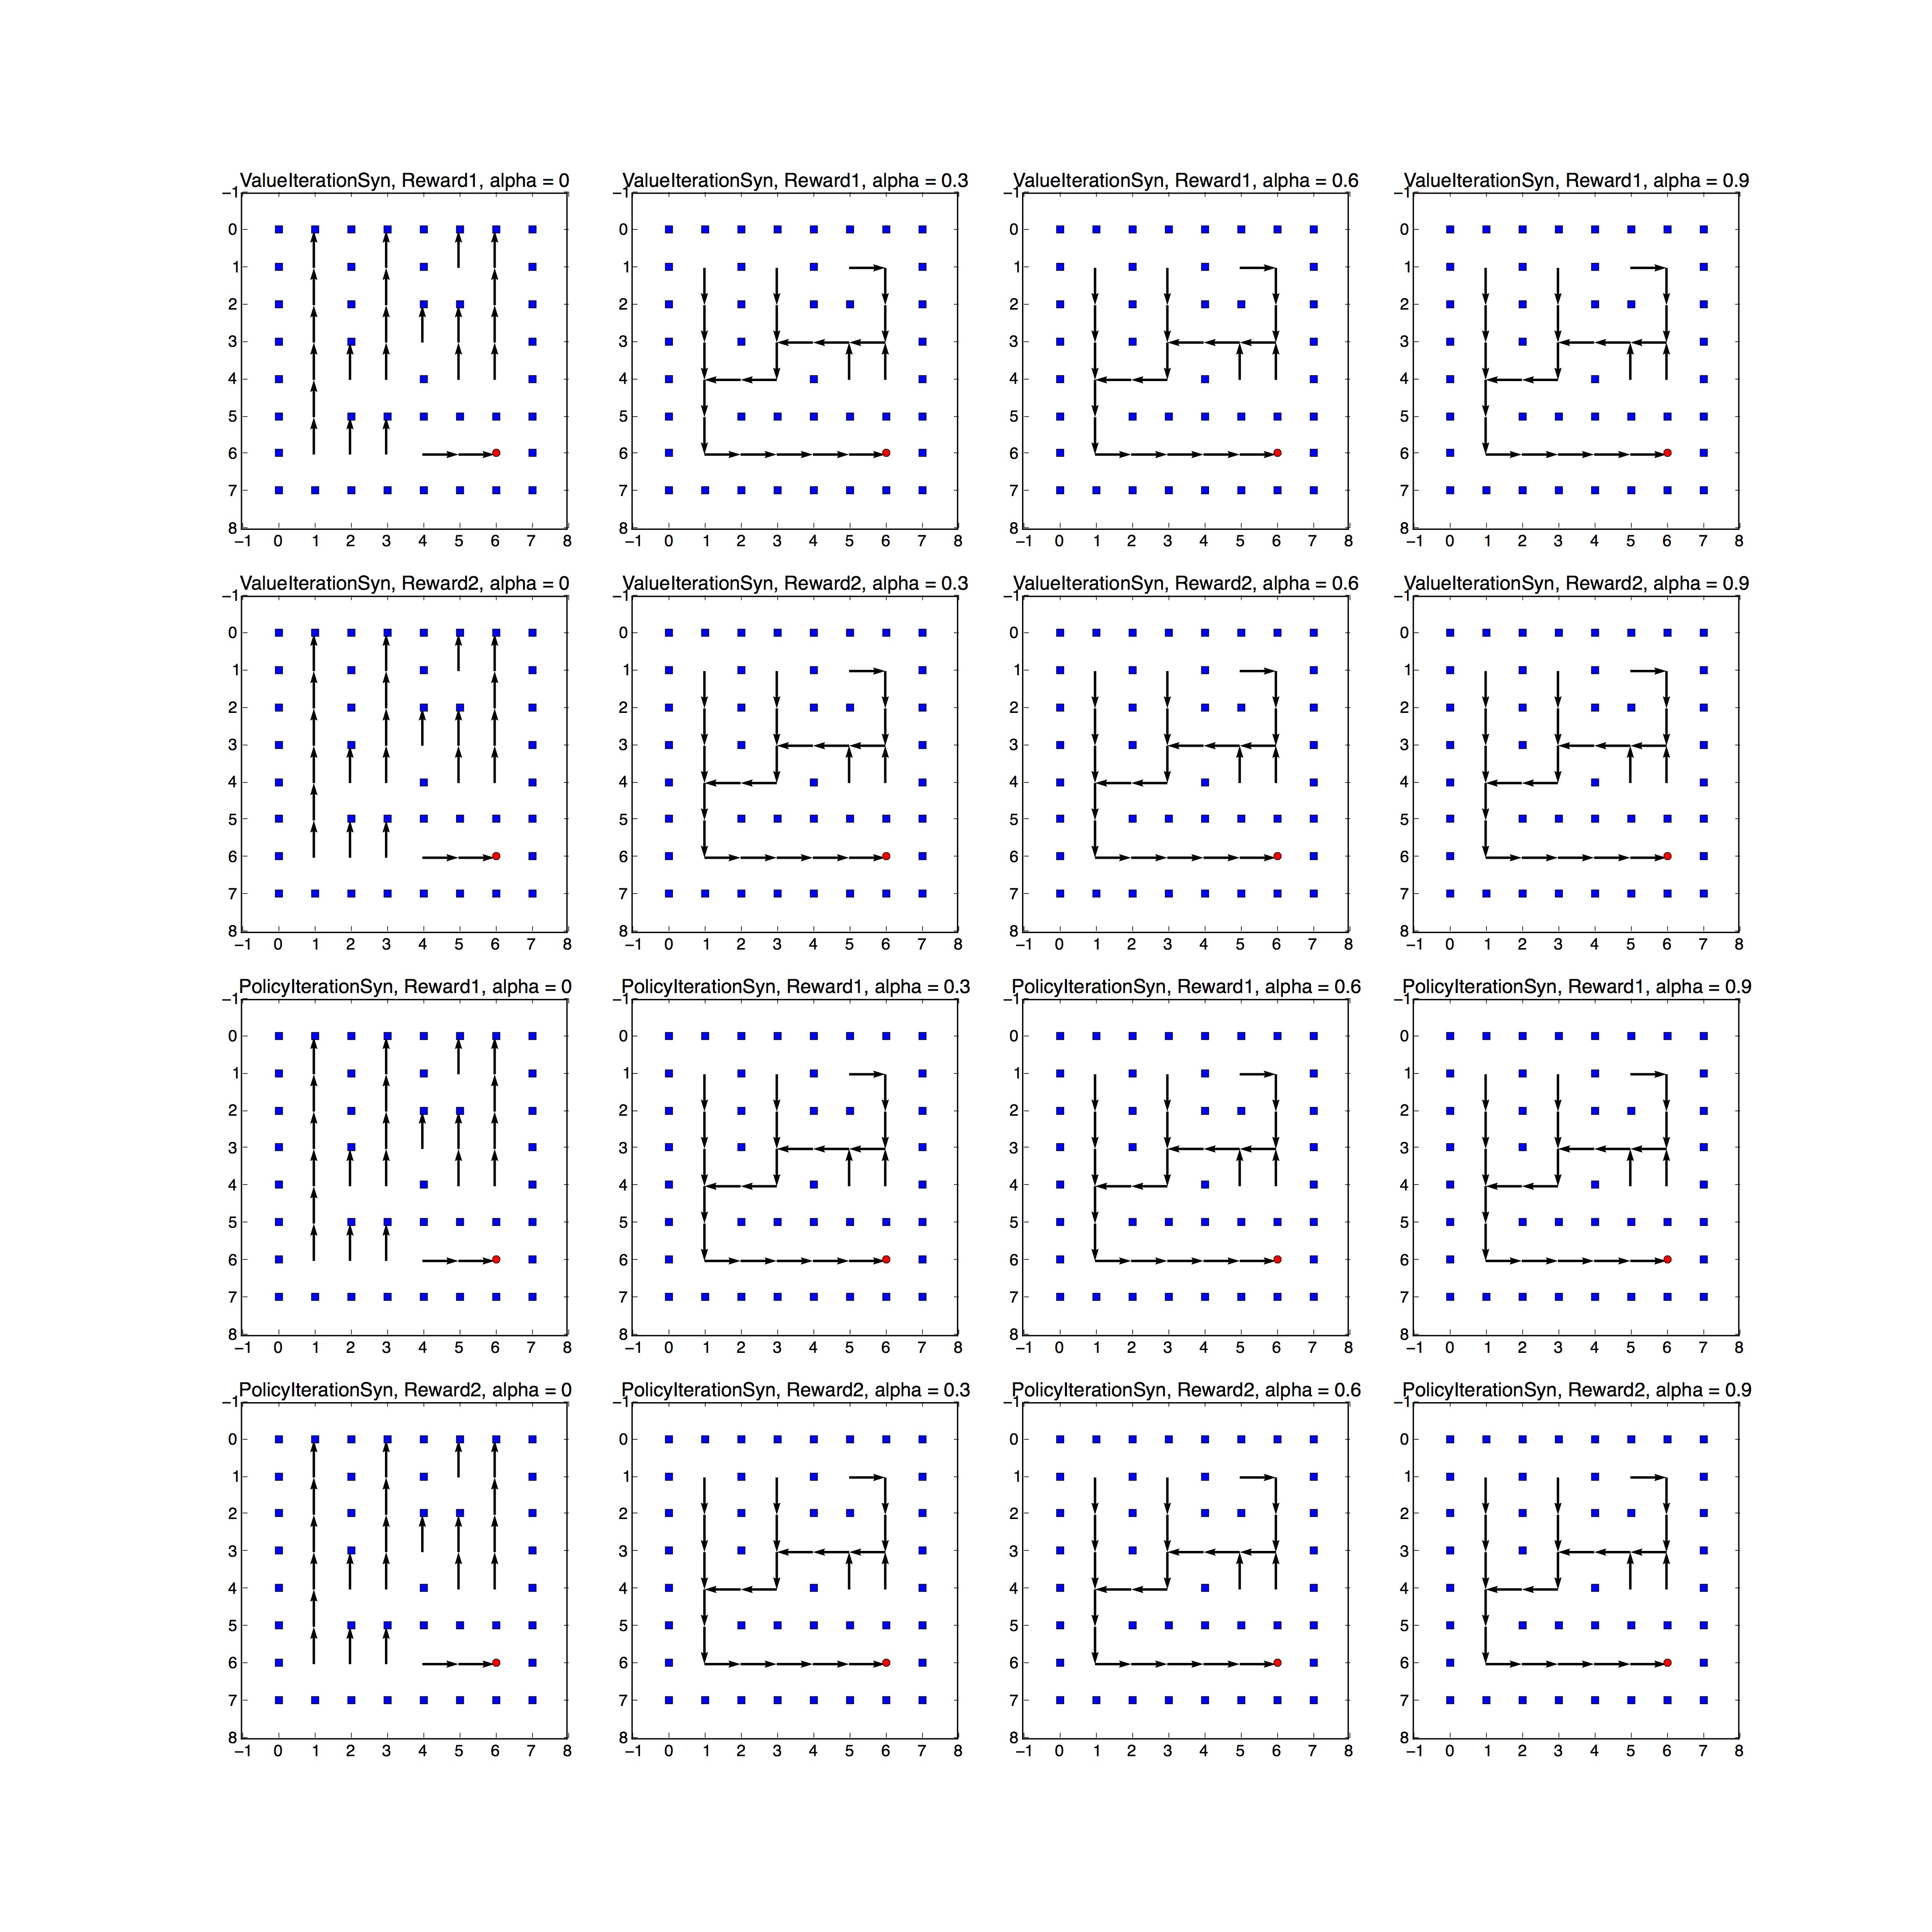
\includegraphics[scale=0.11]{PolicyPlot.jpg}
\end{center}
\newpage
\subsection*{2. Error plots according to different parameter setting}
\begin{center}
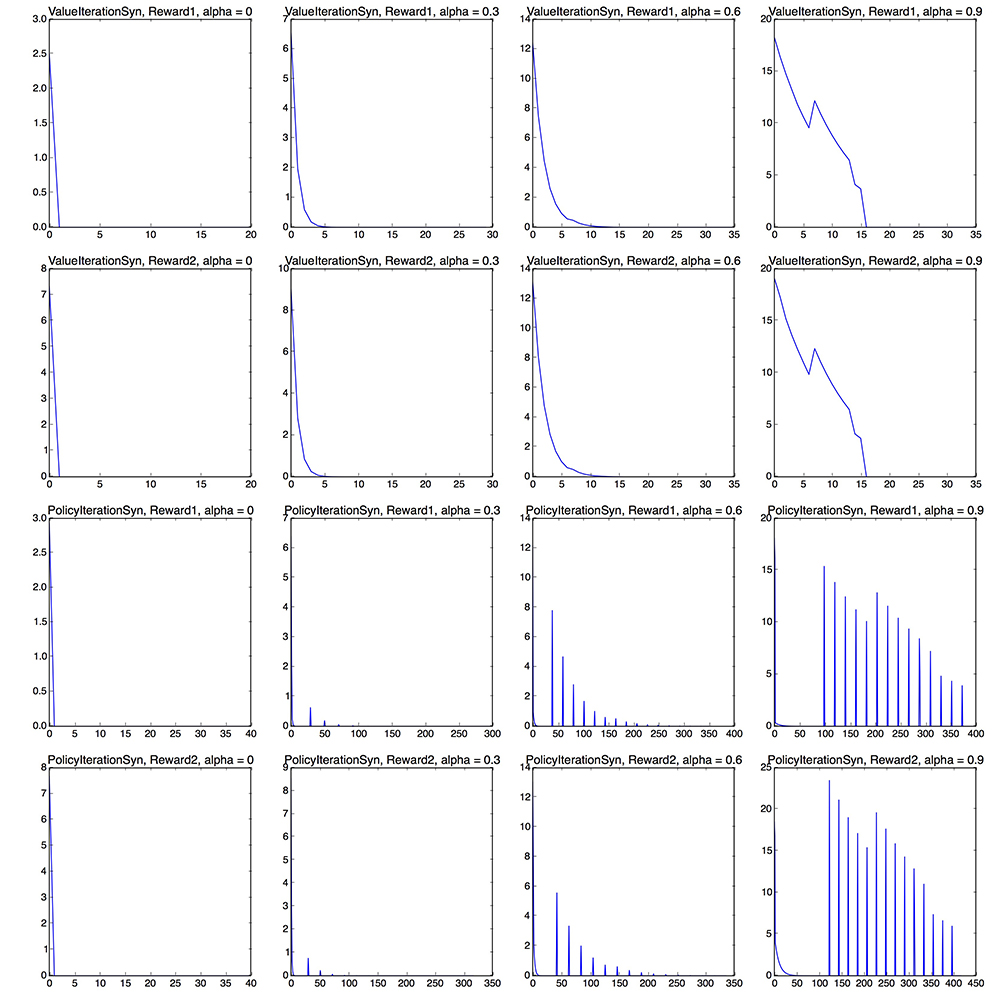
\includegraphics[scale=0.11]{ErrorPlot.jpg}
\end{center}
\newpage
\subsection*{3. Value function plots according to different parameter setting}
\begin{center}
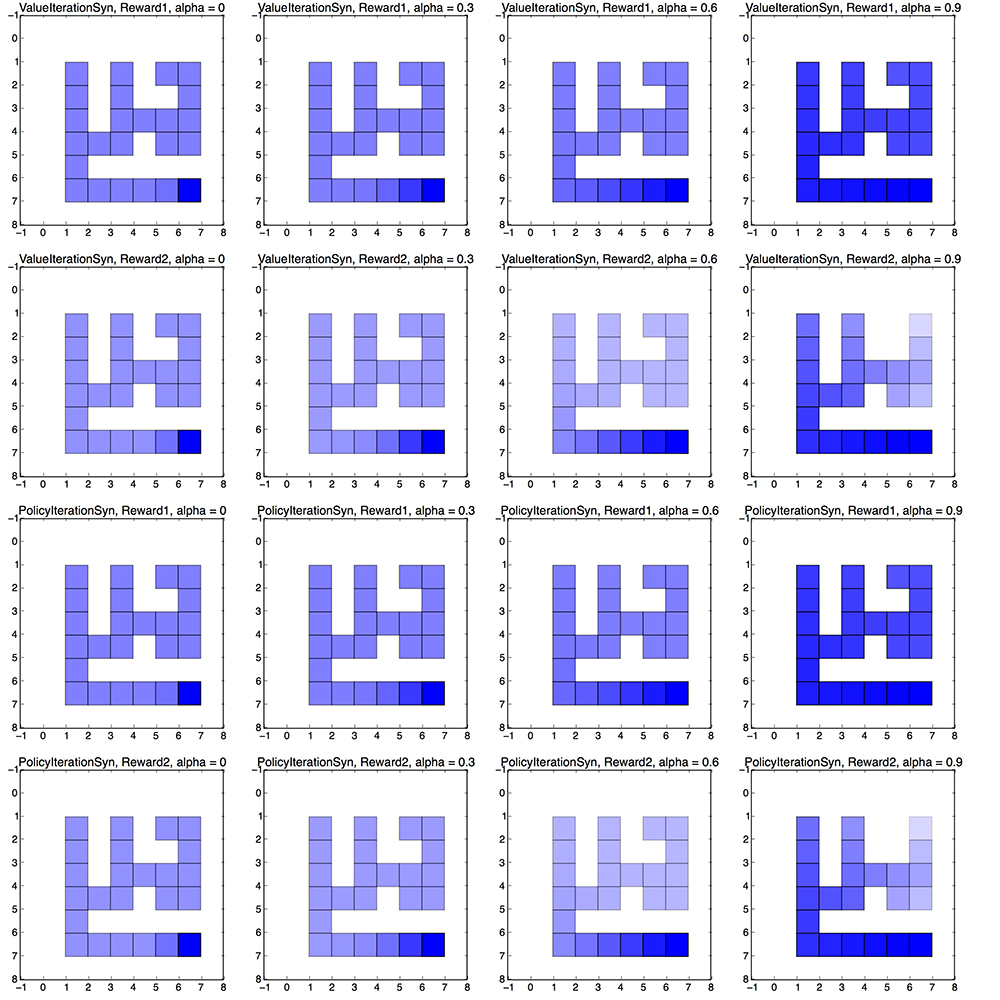
\includegraphics[scale=0.11]{ValueFunctionPlot.jpg}
\end{center}
\end{document}
